\documentclass[margin=1mm]{standalone}
\usepackage[utf8]{inputenc}
\usepackage{amsmath}
\usepackage{amsfonts}
\usepackage{amssymb, bm}
\usepackage{tikz}
\usetikzlibrary{calc,arrows,positioning,shapes,shapes.gates.logic.US,trees, backgrounds}
\usetikzlibrary{fit, positioning}

\begin{document}
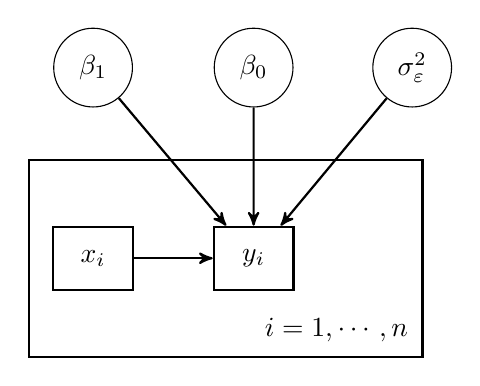
\begin{tikzpicture}[auto,scale=3,
	latent/.style={circle,draw,text badly centered, inner sep=2pt,minimum size=12.5mm},
	error/.style={circle,draw,text badly centered, inner sep=2pt,minimum size=10mm},
	manifest/.style={text centered, rectangle,draw,thick,inner sep=3pt,minimum height=8mm, minimum width=8mm, text width= 8 mm},
	  plate/.style={draw, shape=rectangle,thick, minimum height=2.5cm, minimum width=5cm, text width=1cm, align=right, inner sep=10pt, inner ysep=10pt, append after command={node[above left= 3pt of \tikzlastnode.south east] {#1}}},
	manifestRot/.style={text centered, rectangle, draw, thick,inner sep=3pt, minimum width=7mm, text width= 7mm, minimum height=15},
	manifestfront/.style={rectangle,draw,thick,inner sep=0pt,minimum size=12mm, fill=white},
	ghost/.style={rectangle, inner sep=0pt,text centered,    minimum height=0mm, minimum width=5mm, text width= 5 mm},
	lcorr/.style={<->,>=stealth', bend right=40},
	rcorr/.style={<->,>=stealth', bend left=40},
	fcorr/.style={<->,>=stealth', bend left=40},
	ofcorr/.style={<->,>=stealth', bend right=60},
	ofcorr2/.style={<->,>=stealth', bend left=60},
	intercept/.style={regular polygon,
        regular polygon sides=3,draw,thick,inner sep=0pt,minimum size=10mm},
	mean/.style={regular polygon,regular polygon sides=3,draw,thick,inner sep=0pt,minimum size=10mm},
	paths/.style={->, thick, >=stealth'},
	variance/.style={<->, thick, >=stealth', bend left=270, looseness=2},
	varianceTop/.style={<->, thick, >=stealth', bend right=270, looseness=2},
	unique/.style={<->, thick, >=stealth', loop below=270, looseness=8},
	factvar/.style={<->, thick, >=stealth', loop right=270, looseness=8}
	] % End Creating Path Model Pieces
\tikzset{mystyle/.style={->,double=black}}


% person model
\node [manifest] at (0,0) (x) {$x_{i}$};
\node [manifest] [right = 1cm of x] (y) {$y_{i}$};

\node [error]    [above = 1.5cm of y] (b0) {$\beta_0$};
\node [error]    [above = 1.5cm of x] (b1) {$\beta_1$};
\node [error]    [right = 1cm of b0] (e) {$\sigma^2_{\varepsilon}$};
\node [plate={$i=1, \cdots, n$}] [right= -1.35cm of x, yshift=0cm] (p) {};

% paths
\draw[paths] (x)  -- (y);
\draw[paths] (b0) -- (y.north);
\draw[paths] (b1) -- (y);
\draw[paths] (e)  -- (y);


\end{tikzpicture}
\end{document}